\chapter{Introduction}\label{ch:introduction}

\section{Context}

Artificial intelligence has rapidly advanced through Large Language Models (LLMs), which demonstrate remarkable abilities in natural language understanding, reasoning, and instruction following \cite{minaeeLargeLanguageModels2025, zhaoSurveyLargeLanguage2025}. These models have fundamentally changed how we think about AI systems, showing that scaling up neural networks trained on massive text corpora can unlock emergent capabilities ranging from code generation to complex reasoning.

Recently, researchers have extended this paradigm to create vision-language models that integrate text and vision, enabling systems that not only converse but also see \cite{caffagniRevolutionMultimodalLarge2024, liSurveyStateArt2025}. This represents a crucial step toward more general AI systems that can interact with the real world through multiple modalities. Visual-language assistants demonstrate that the reasoning capabilities of LLMs can be successfully grounded in visual perception, opening new possibilities for AI applications.

Understanding how these models integrate modalities is crucial not only for improving performance, but also for ensuring robustness, transparency, and trustworthiness. As these systems become more capable, we need to understand their internal mechanisms to ensure they behave reliably and can be debugged when they fail.

\textsc{LLaVA} (Large Language and Vision Assistant) \cite{liuVisualInstructionTuning2023, liuImprovedBaselinesVisual2024} represents a breakthrough in vision-language modeling: a vision encoder feeds a projector that maps visual features into an LLM backbone (see Figure~\ref{fig:llava_architecture}), enabling image-grounded dialogue after instruction tuning. LLaVA acquires its visual instruction-following ability in two stages: (i) a projection layer is learned to align vision features with the LLM's embedding space while leaving the backbone unchanged; (ii) \emph{visual instruction tuning} fine-tunes the projector and backbone (with the vision encoder frozen) on image-text instruction-response pairs, equipping the system to follow image-grounded instructions. While the success of LLaVA on visual instruction following benchmarks is well-documented \cite{liuVisualInstructionTuning2023, liuImprovedBaselinesVisual2024}, we lack a precise account of where and how visual instruction tuning alters the LLM backbone itself to enable LLaVA to follow image-grounded instructions, and whether these changes differ between text-only and multimodal inputs.

\begin{figure}[h]
    \centering
    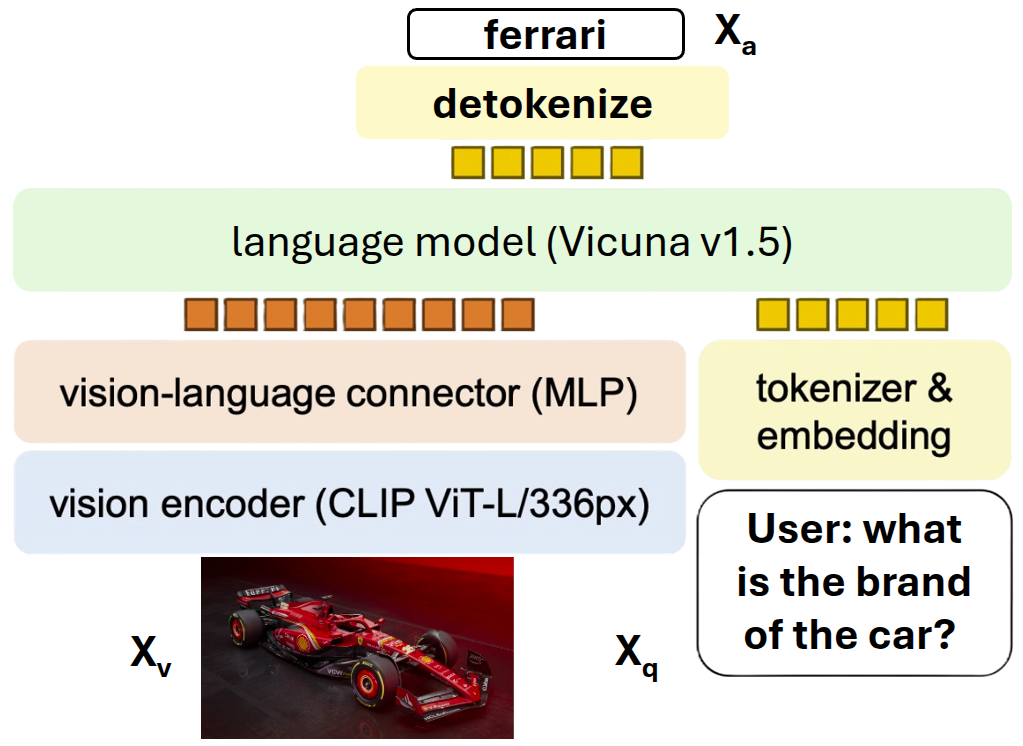
\includegraphics[width=0.6\textwidth]{../images/chapter1/llava_architecture.png}
    \caption{
        LLaVA v1.5 architecture. 
        The model consists of a vision encoder (CLIP-ViT-L-336px) \cite{radfordLearningTransferableVisual2021}, a language model backbone (Vicuna v1.5) \cite{vicuna2023}, and an MLP projection layer.
        Adapted from \cite{liuImprovedBaselinesVisual2024}.
    }
    \label{fig:llava_architecture}
\end{figure}

\section{Research Problem and Motivation}

While the alignment stage updates only the projection layer, the fine-tuning stage modifies the language-model backbone itself. This two-stage training setup raises a fundamental question:

\begin{quote}
\textbf{How does visual instruction fine-tuning change the internal representations of LLaVA's backbone, and where in the depth of the network do these changes concentrate?}
\end{quote}

This thesis addresses this question.

From an interpretability perspective, it is crucial to identify which parts of the backbone support visual reasoning and how they change under fine-tuning. In practice, this understanding enables performance improvements while preserving core language abilities and enhancing robustness across tasks and inputs. Localizing where changes concentrate enables more efficient training such as targeting specific layers instead of end-to-end updates. Ultimately, understanding how internal representations develop is essential for safe and reliable deployment on downstream tasks.

\section{Contributions}

This work makes four key contributions to the understanding of the impact of vision instruction fine-tuning in LLaVA:

\begin{enumerate}
    \item \textbf{Layer-localized representational analysis}: Through representational similarity measures such as Neighborhood Overlap and Linear CKA, we quantify that the LLaVA backbone changes most in the early-mid layers with partial convergence to the equivalent representational similarity between text-only and multimodal inputs in deep layers in question answering tasks.
    
    \item \textbf{Geometric characterization}: We compare the geometry of the representations before and after fine-tuning and demonstrate that fine-tuning compresses mid-layer geometry (lower intrinsic dimension and entropy), especially for multimodal inputs.
    
    \item \textbf{Modality-gap analysis}: Given the importance of textual and visual modality integration in multimodal models for tasks such as multimodal retrieval, we measure how the geometric separation between text and image representations or \emph{modality gap} evolves with depth and how fine-tuning shifts that gap across different tasks.
    
    \item \textbf{Functional validation via layer patching}: We show that patching early-mid fine-tuned layers into the pretrained backbone recovers most performance gains, while late layers yield diminishing returns.
\end{enumerate}

\section{Thesis Structure}

The remainder of the thesis is organized as follows. Chapter~\ref{ch:literature_review} provides a review on instruction-tuned LLMs, vision-language models, the LLaVA architecture and its training paradigm, and the theoretical foundations for our analysis methods. Chapter~\ref{ch:methodology} details our experimental approach, including datasets, similarity measures, geometric analysis tools, and the layer patching protocol. Chapter~\ref{ch:results_and_discussion} presents our findings on representation similarity, geometric reorganization, modalities alignment, and functional validation through layer patching. Chapter~\ref{ch:conclusions} summarizes our key findings, discusses their implications, acknowledges limitations, and outlines directions for future research.
